David Rohrbaugh

2015-03-15

Spring Break and the weeks before and after (3/9 - 3/27)

\begin{tabular}{|p{5cm}|p{5cm}|}
 \hline
 Week of 3/9&
 This week we tested different launching mechanisms with different materials to try to improve on the design we used for the State tournament. None of them worked very well consistently, and none were able to launch big balls as well as our previous design.\\
\hline
 Week of 3/16&
 This week we decided to reattach our old launching mechanism as it was the best mechanism we had tested so far. The robot is coming together again as the Super-Regional tournament approaches. We also made about 470 buttons at FRC Team 4499 The Highlander's shop to distribute at the tournament.\\
\hline
 Week of 3/23&
 This week we did final testing of our robot design and wrote a better autonomous on Monday and Tuesday. On Wednesday, we packed everything up. Thursday after school we flew to Oakland, California.\\
 \hline
\end{tabular}

\medskip

Here are some calculations we ran about our launching mechanism:

The big, middle, and small gears are running at 120, 360, and 720 rpm, respectively. The diameter of our launcher is 11.75 inches. Therefore we can find the circumference with the following calculation:

C = \pi d = 11.75\pi = 36.914 inches

\pagebreak

Here are some images of our launcher prototypes:

\begin{center}
 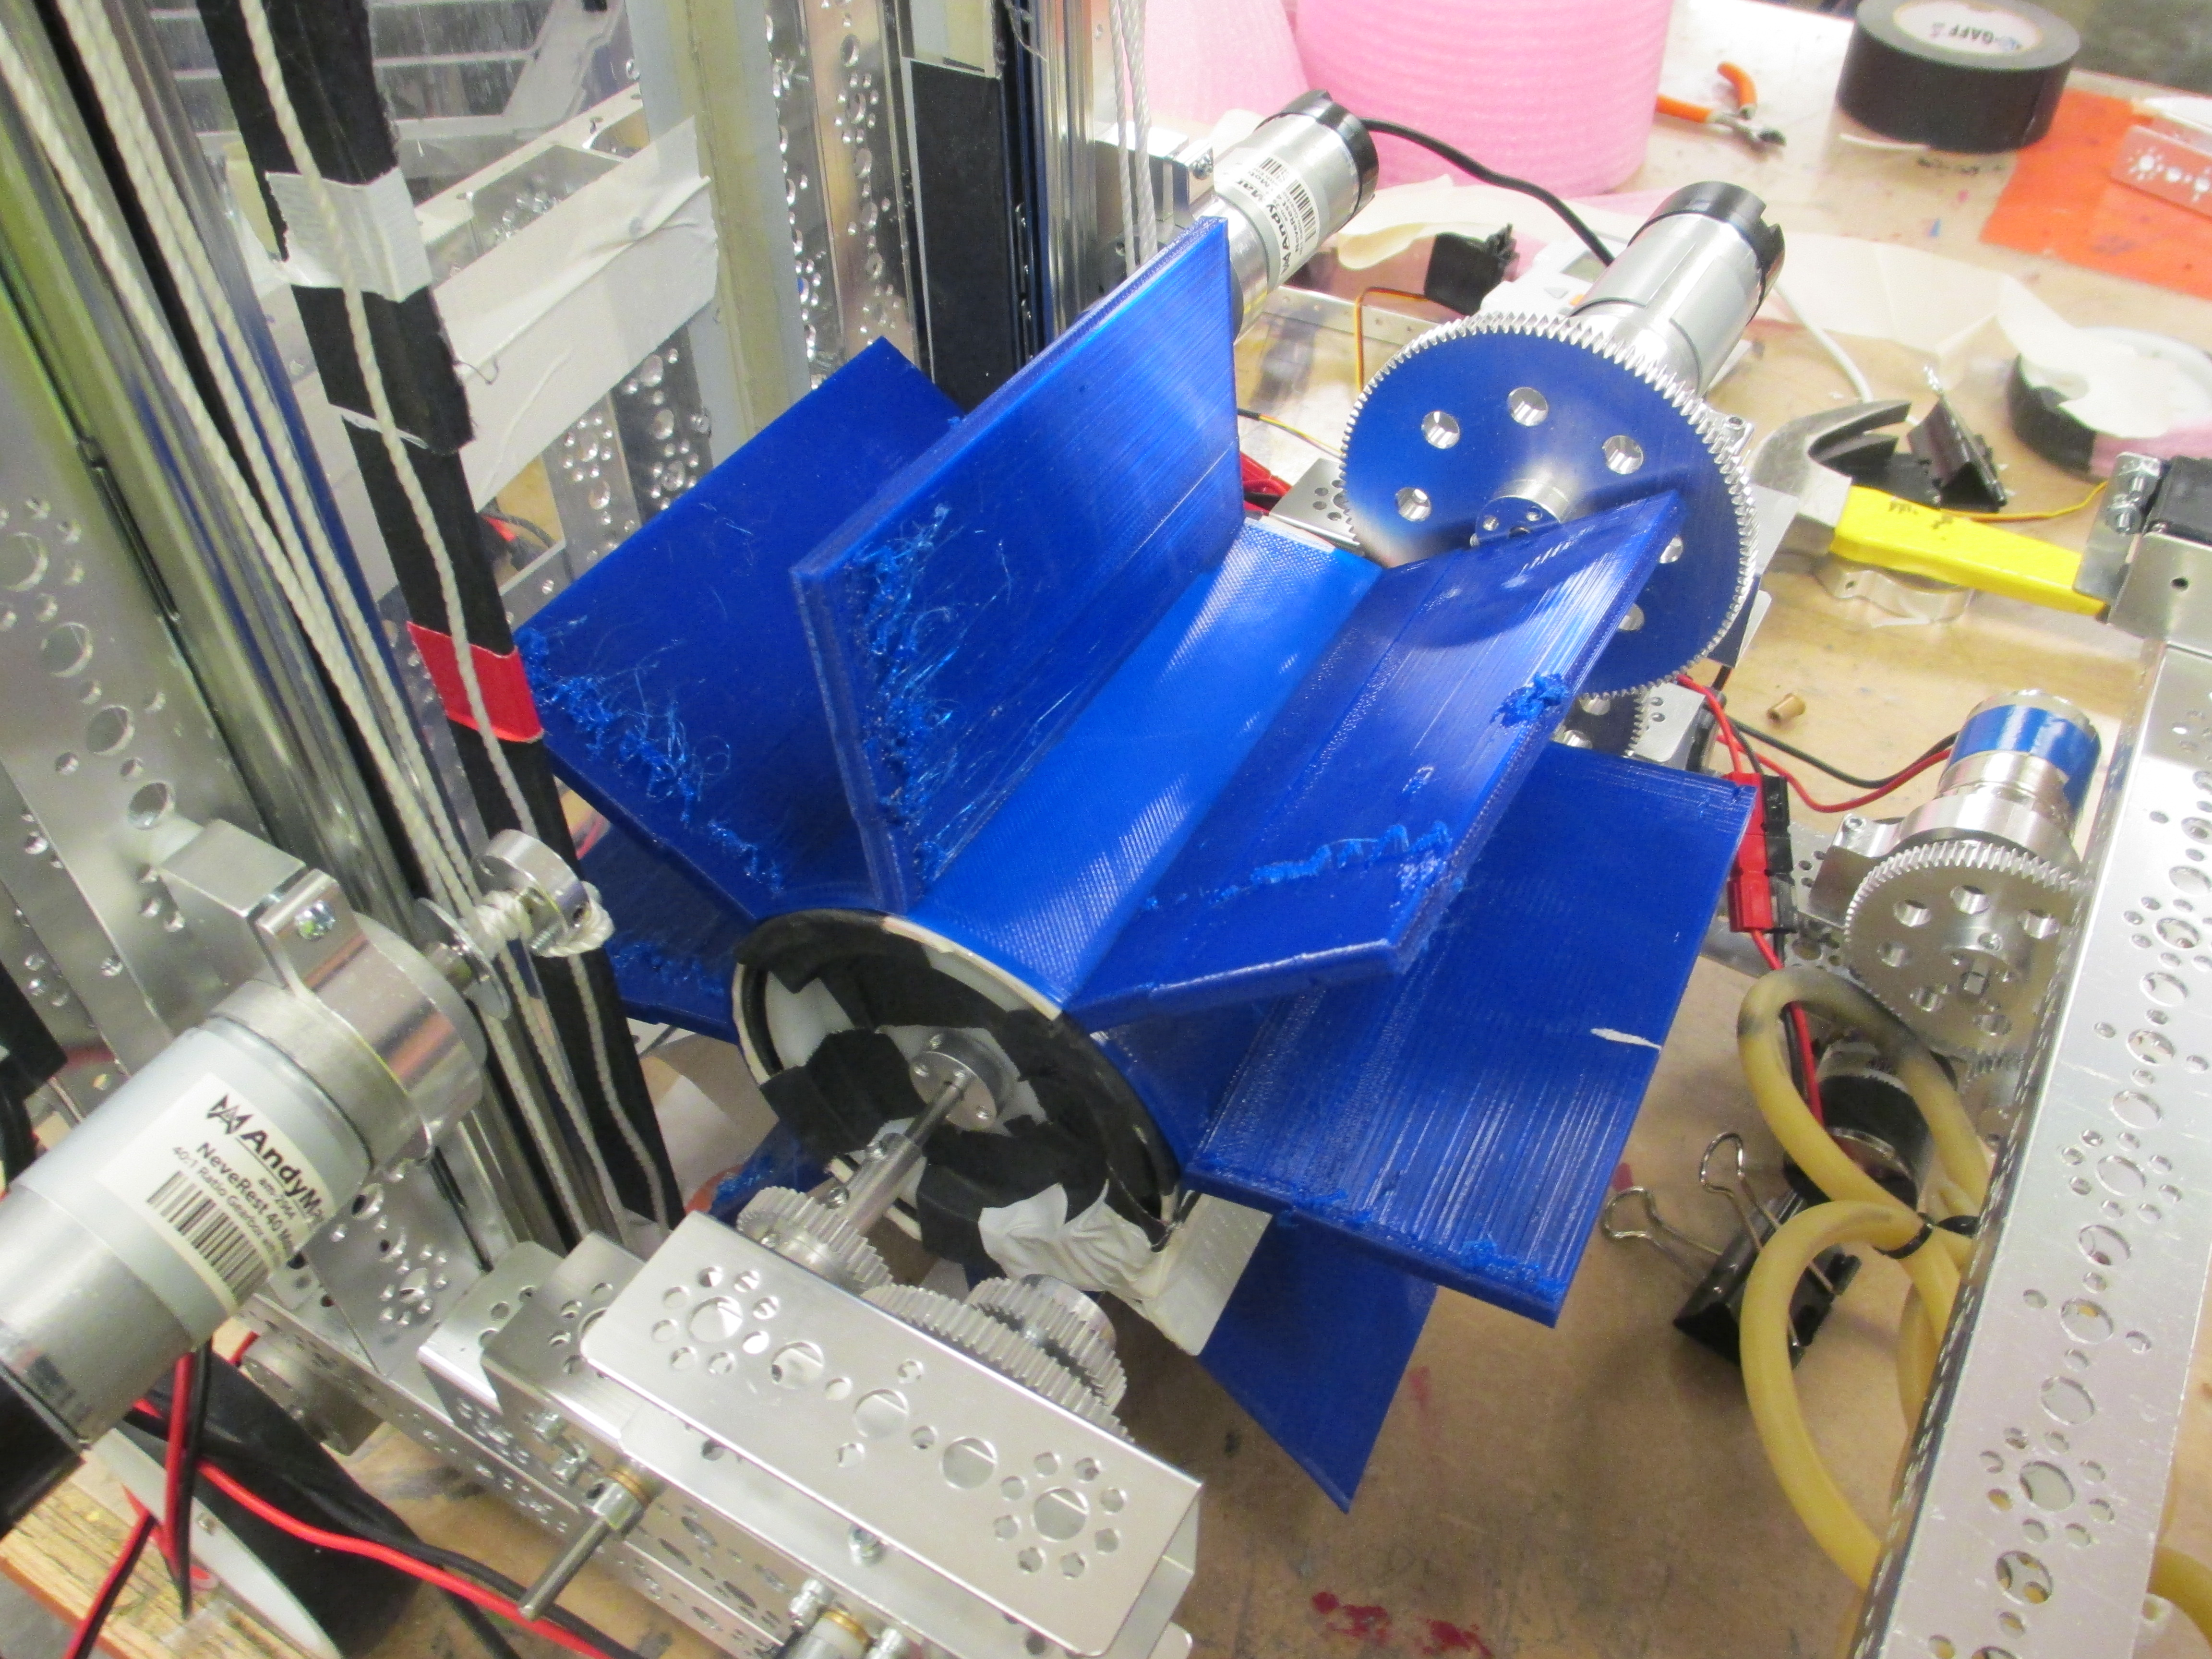
\includegraphics[width=\textwidth]{./Entries/Images/launchProto7.JPG}
\end{center}

\begin{center}
 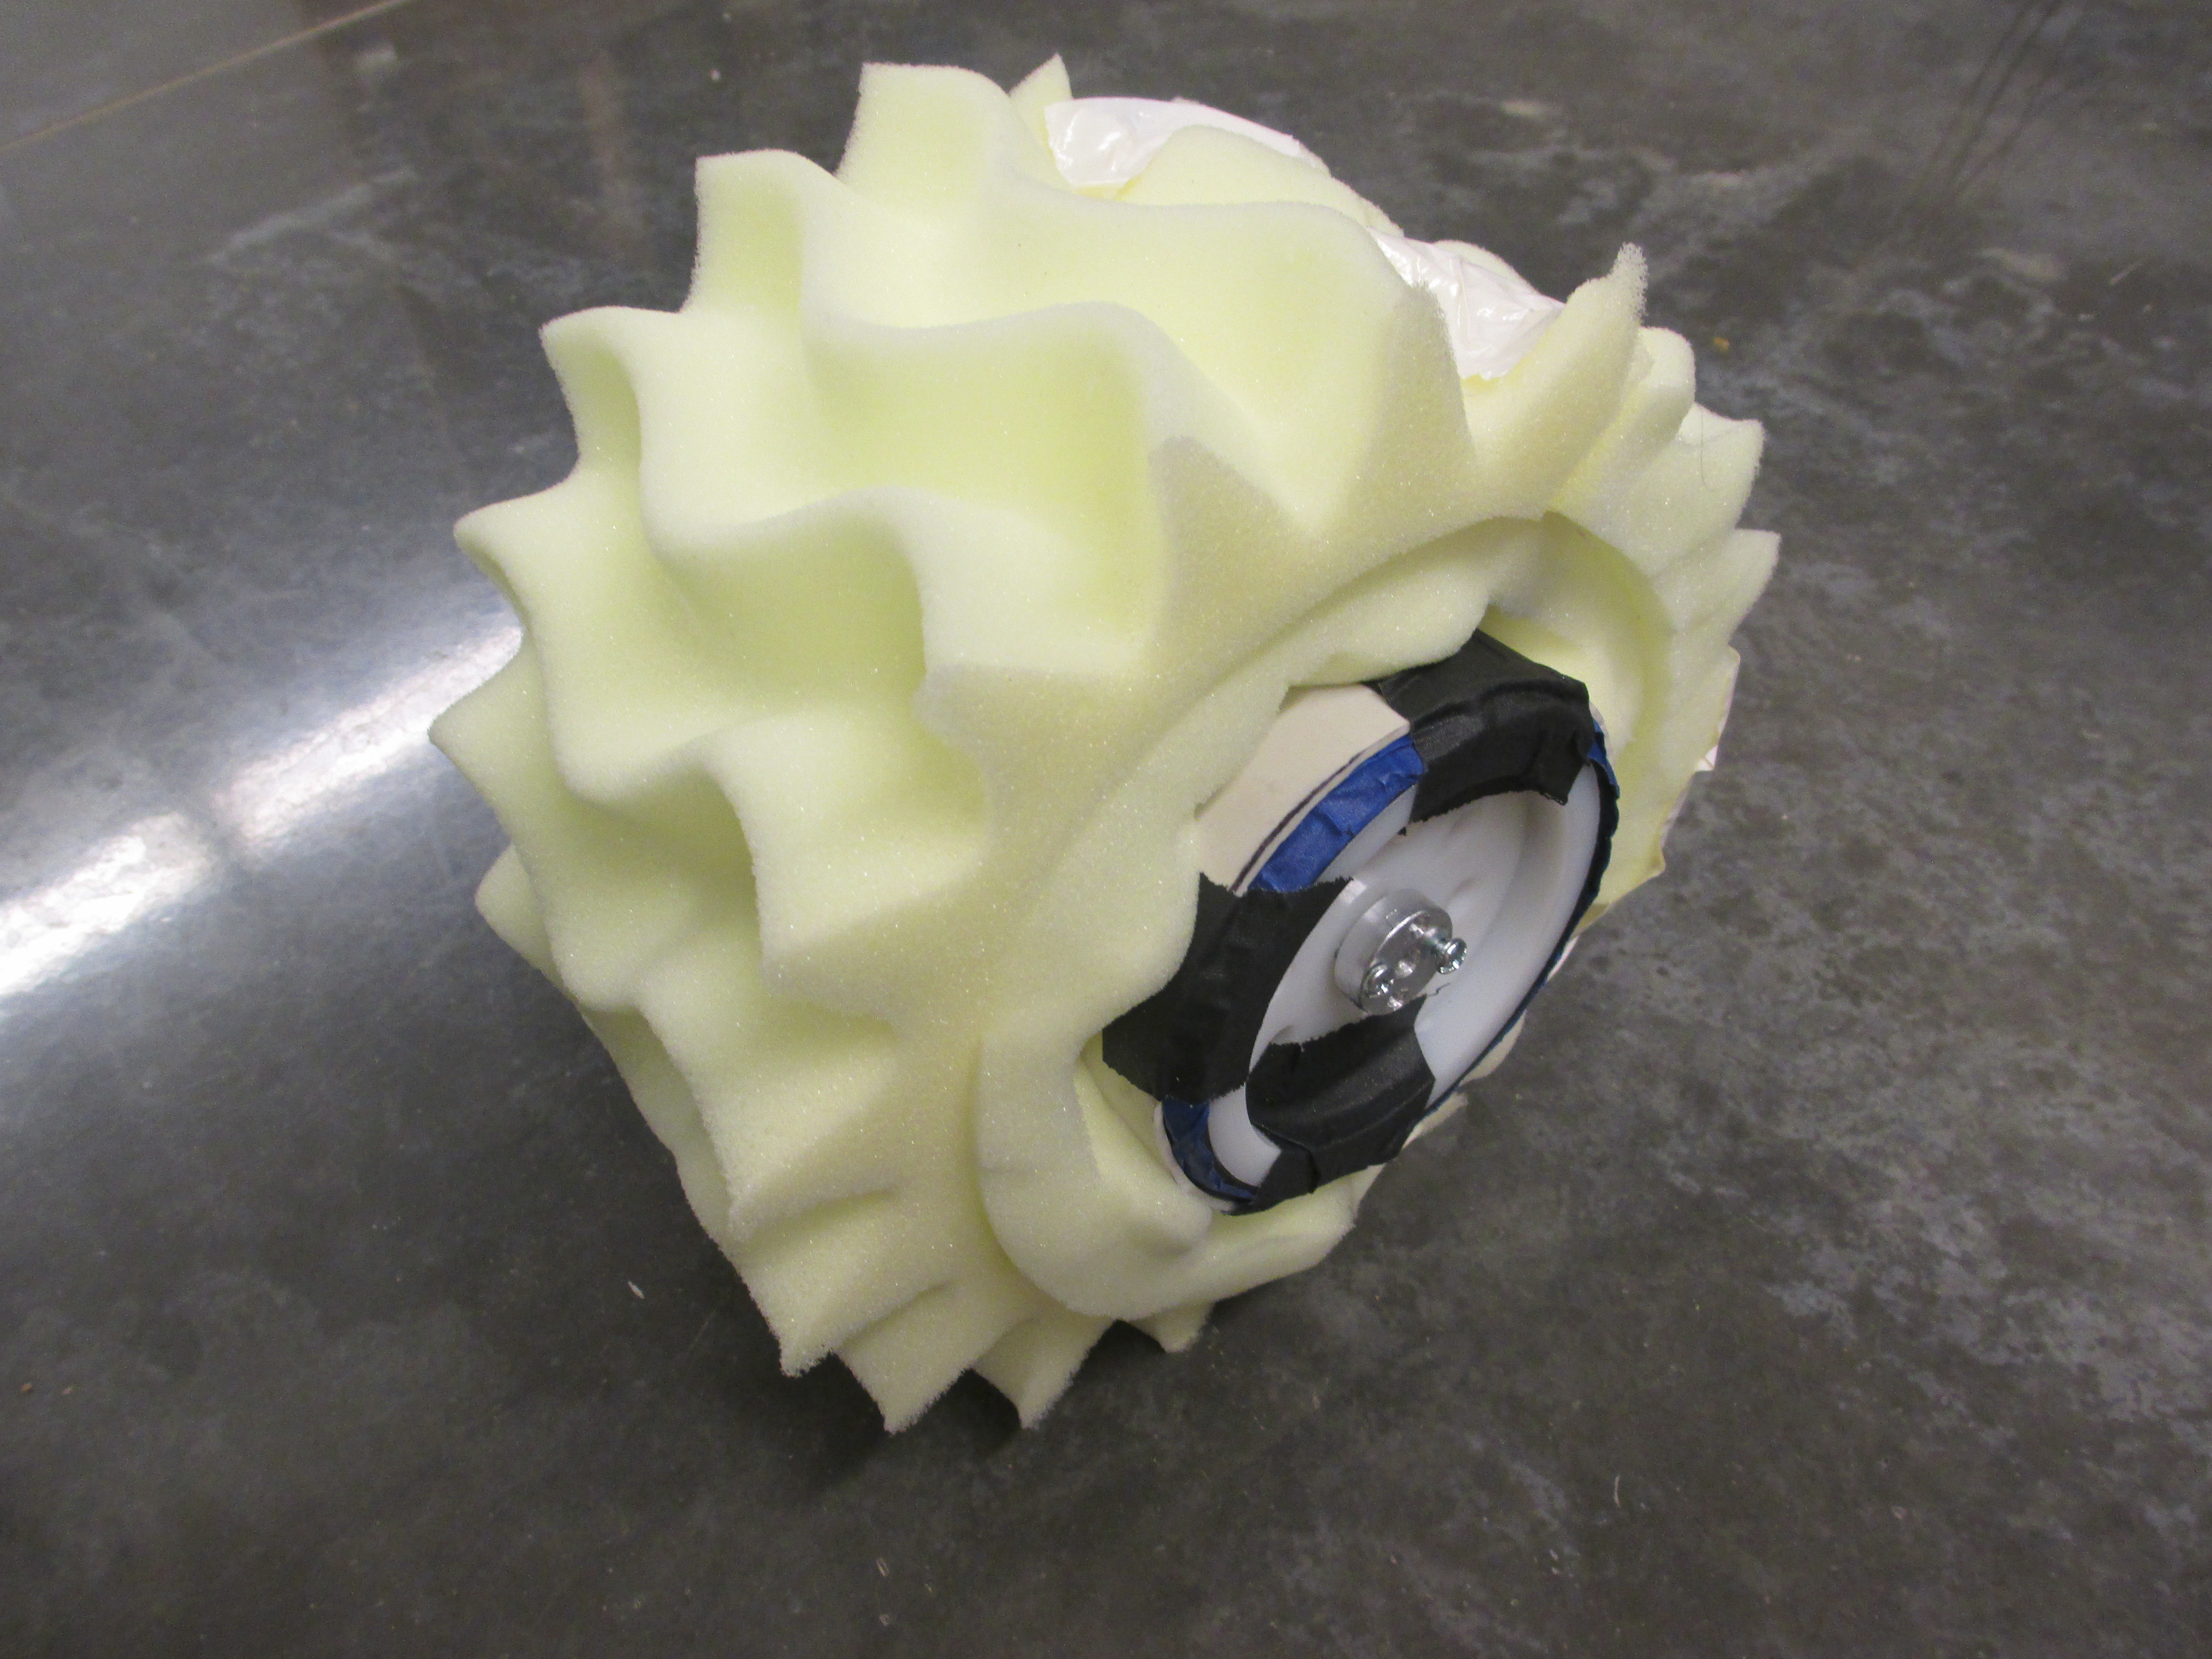
\includegraphics[width=\textwidth]{./Entries/Images/launchProto2.JPG}
\end{center}

\begin{center}
 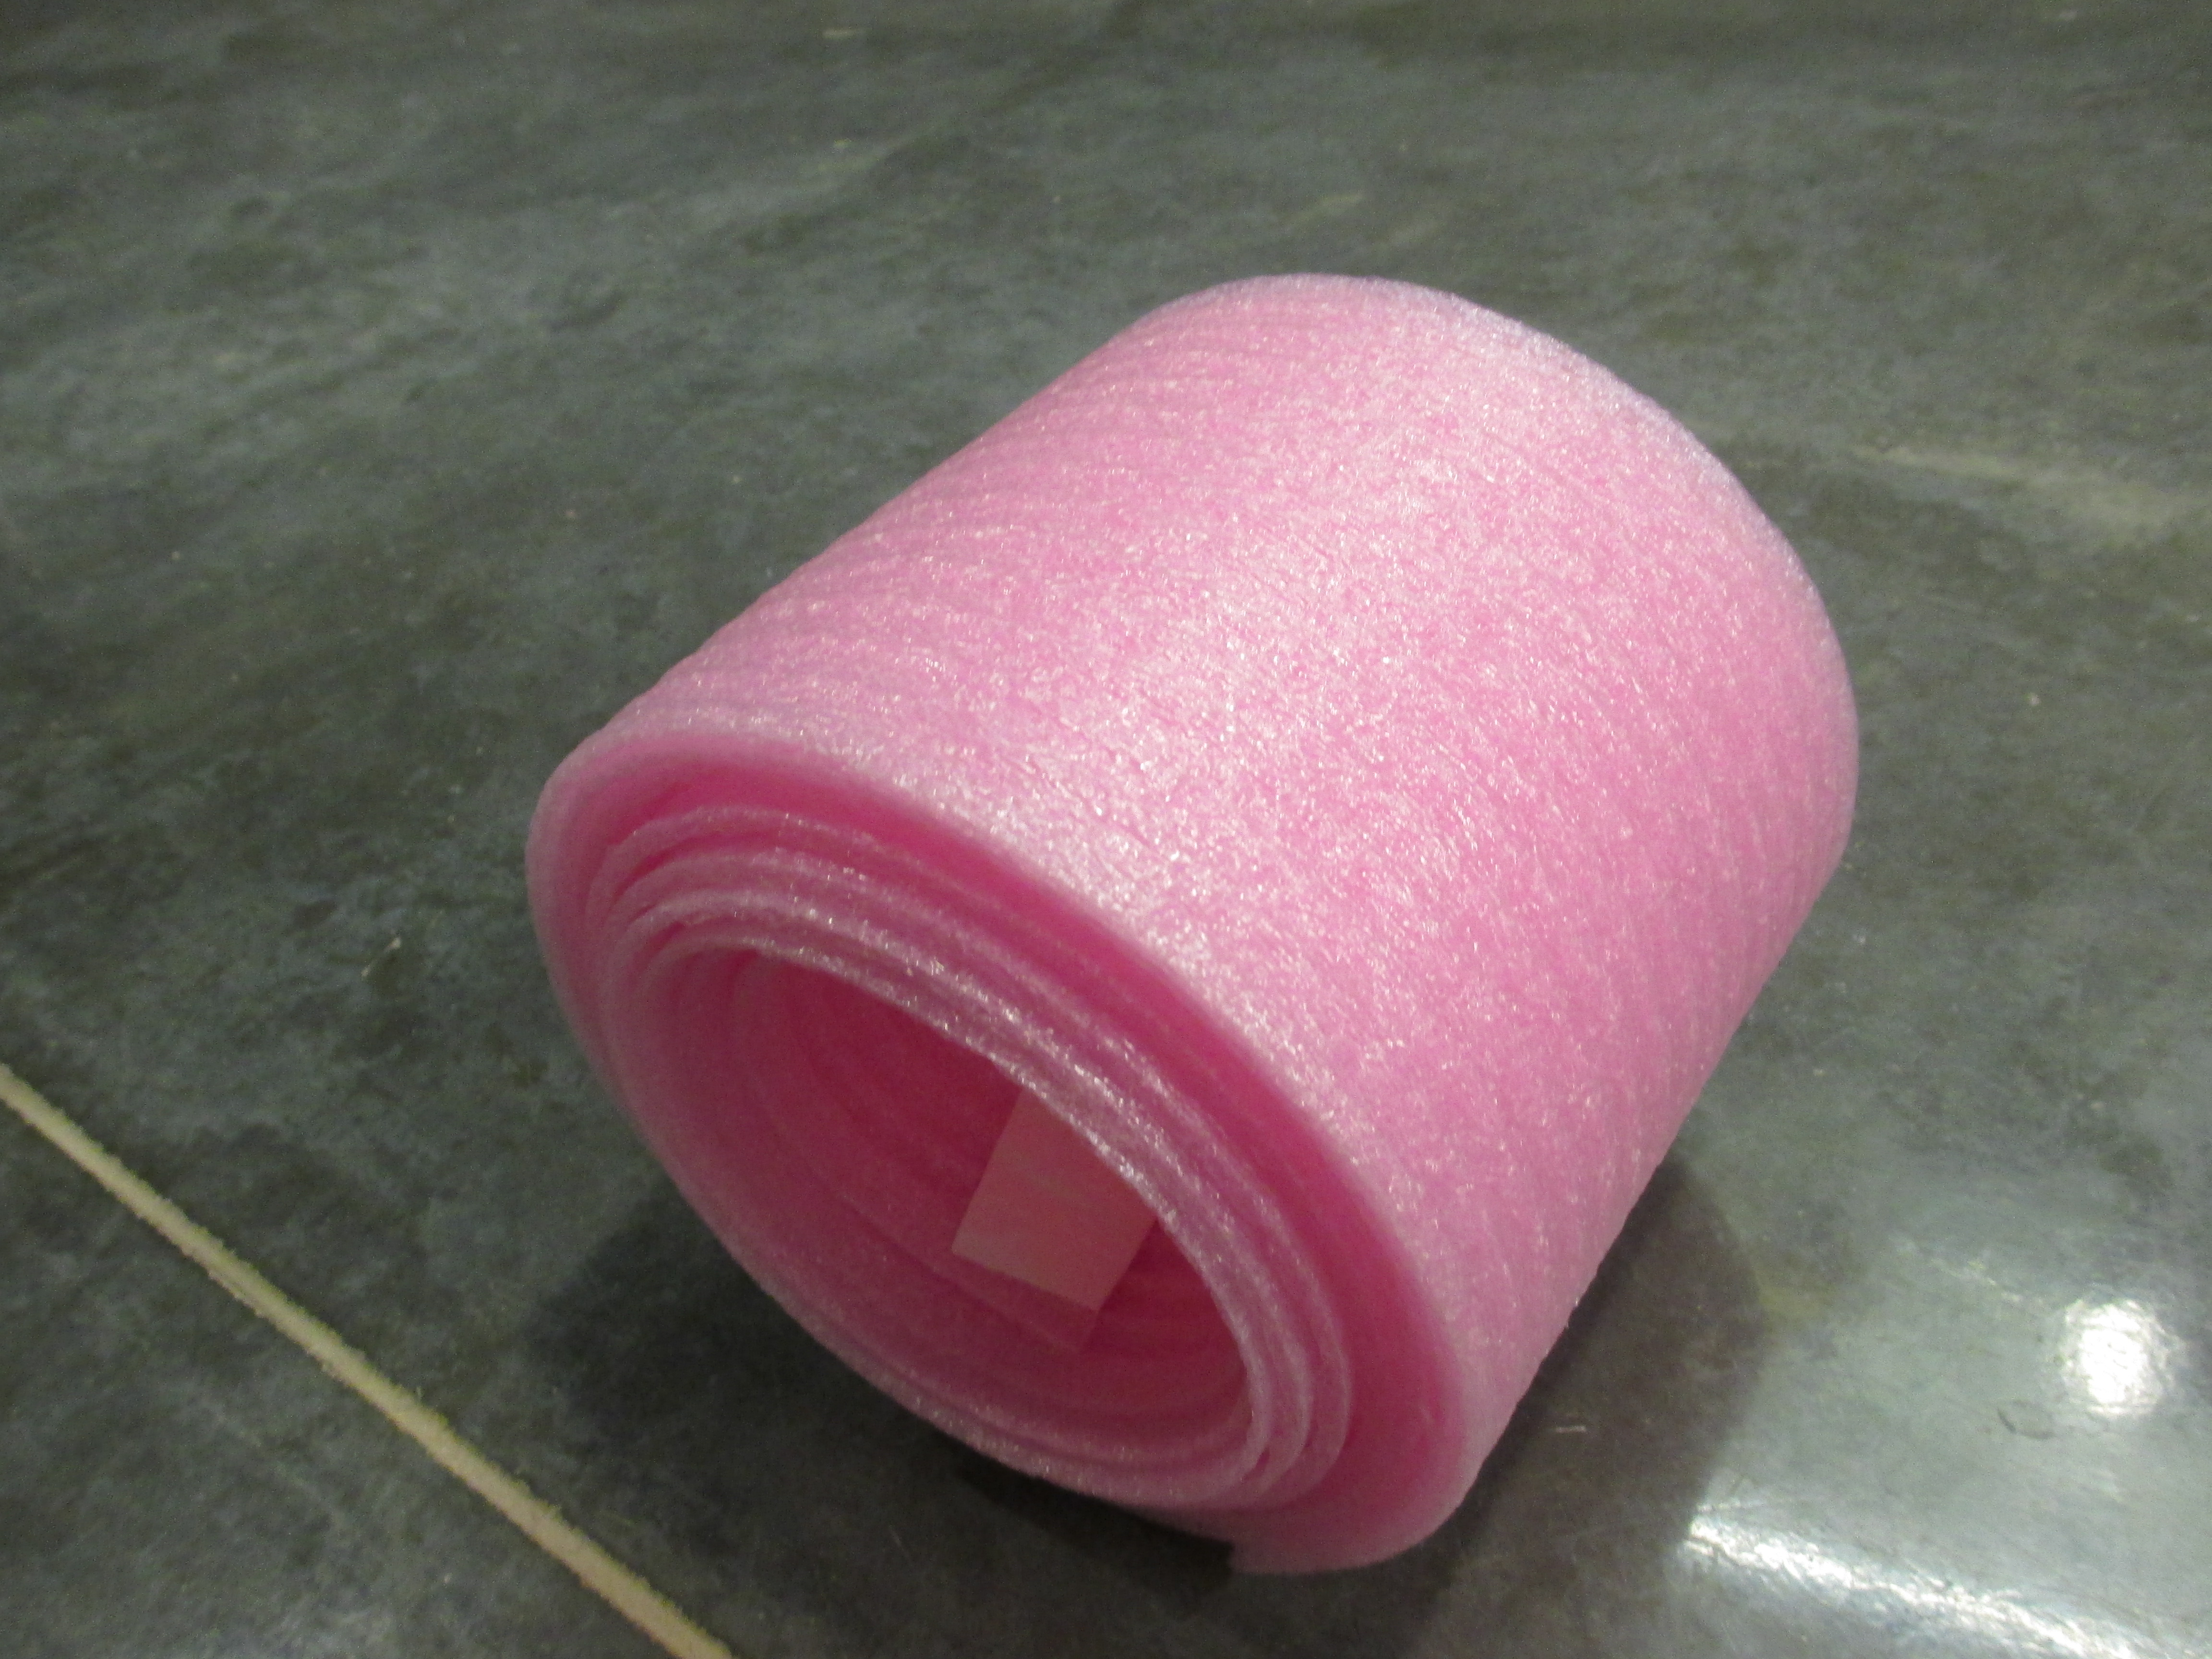
\includegraphics[width=\textwidth]{./Entries/Images/launchProto12.JPG}
\end{center}

%\pagebreak

Oh yeah, and we somehow melted wood...

\begin{center}
 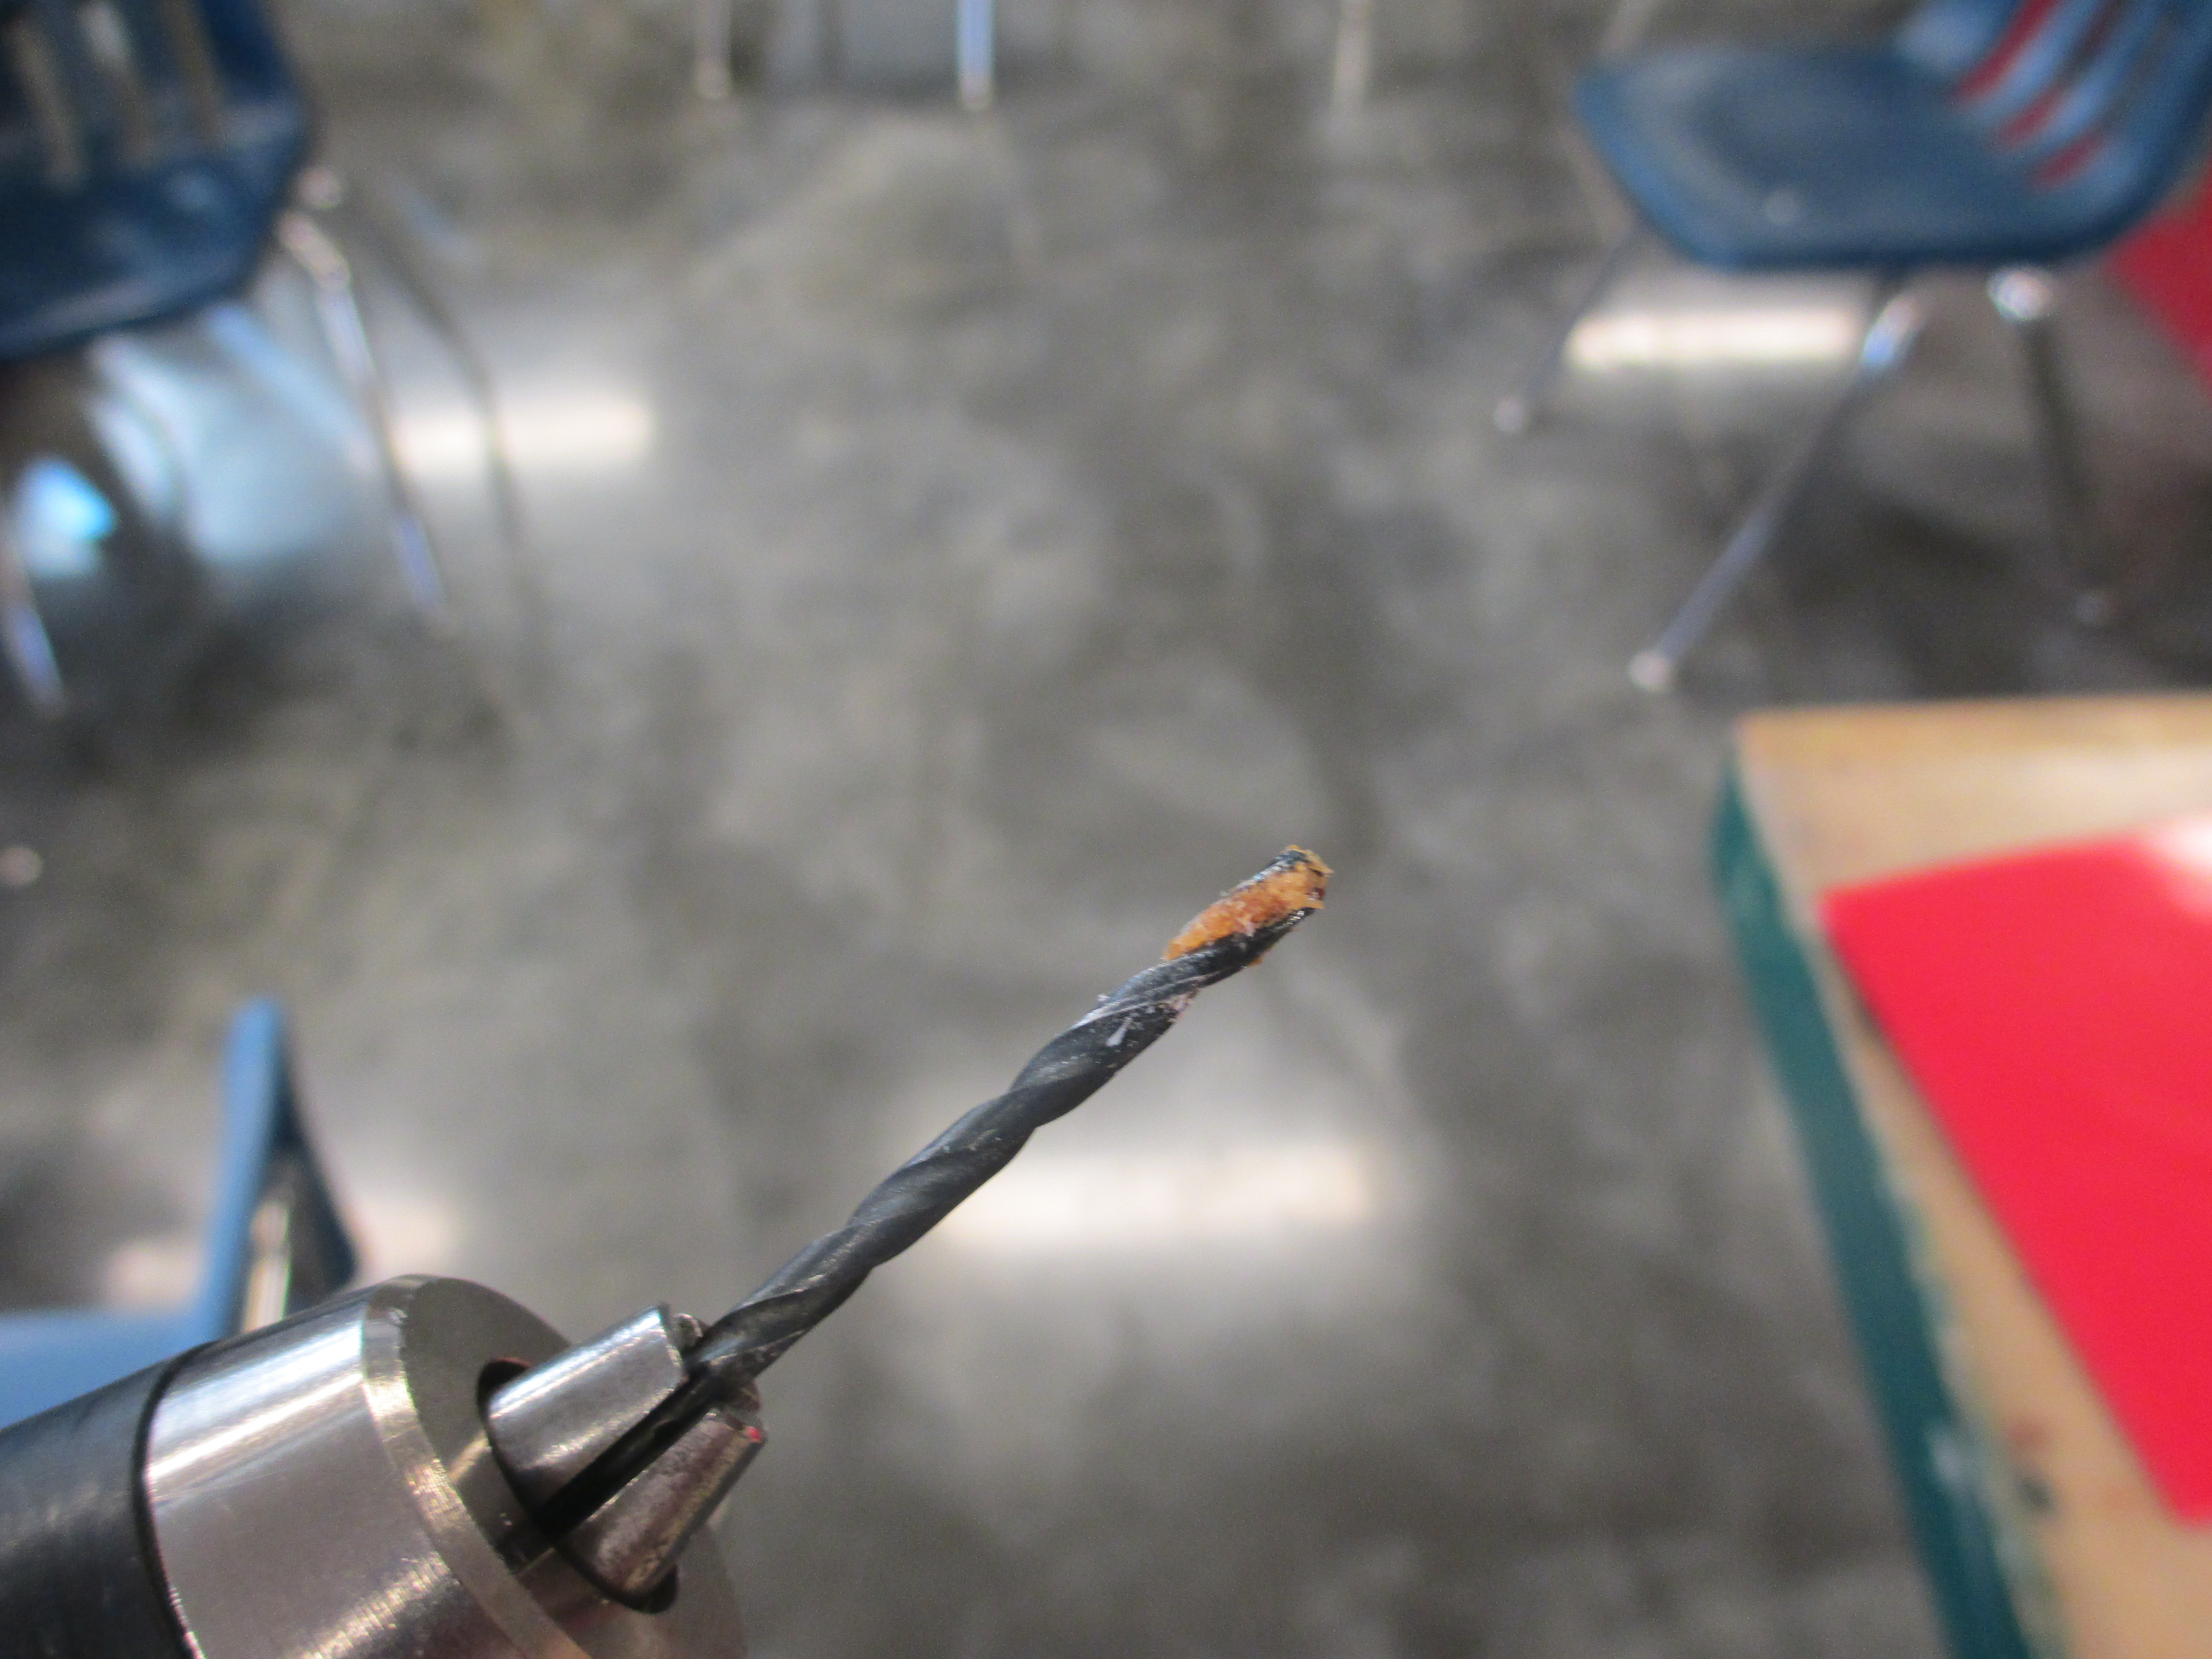
\includegraphics[width=\textwidth]{./Entries/Images/meltedWood.JPG}
\end{center}

...four times.